\documentclass[12pt]{article}

\usepackage[margin=1in]{geometry}
\usepackage{setspace}
\usepackage{graphicx}
\usepackage{float}
\usepackage{amsmath}
\usepackage{booktabs}
\usepackage{hyperref}
\usepackage[backend=biber,style=numeric]{biblatex}
\addbibresource{../docs/references.bib}

\title{The Association Between the Kaitz Index and Employment in Puerto Rico}
\author{Alejandro M. Ouslan \\ \small{University of Puerto Rico, Mayaguez} \\ \small{\texttt{alejandro.ouslan@upr.edu}}}
\date{May 14, 2025}

\begin{document}

\maketitle

\singlespacing

\begin{abstract}
	\textit{
		This study examines the relationship between the Kaitz Index and employment levels in Puerto Rico using panel data at the
		postal code level. The data covers the period from Q1 2012 to Q4 2023. A Spatial Durbin Model with fixed effects is applied
		to investigate both the direct effect of the Kaitz Index on employment and potential spatial effects from adjacent regions.
		The findings largely support existing literature suggesting a negative relationship between the minimum wage and employment.
		Additionally, despite some convergence issues with the MCMC of the Kaitz variable, the confidence interval indicates a
		negative spillover effect on neighboring regions’ employment levels.
	}
\end{abstract}

\section{Introduction}

The minimum wage and its impact on employment are among the most debated topics in labor economics, especially in regions with
unique economic structures like Puerto Rico. Numerous studies have attempted to analyze this relationship, yielding diverse
results. For example, a meta-analysis by Stanley (2009) \cite{doucouliagos2009publication} and Card \& Krueger (1994) \cite{card1994comment} concluded that there is no significant
effect on employment, while the Federal Reserve's 2012 \textit{Competitiveness of the Puerto Rican Economy} (2012) \cite{torres2012competitividad} report emphasized
the need for policies that focus on employment creation and suggested a subminimum wage for young workers under 25. Locally,
Hernández (2017) found a reduction in total employment following minimum wage increases, while Hernández \& Wu (2025)
identified differential responses by local versus foreign-owned businesses. However, the spatial dynamics of the minimum
wage—how wage conditions in one region may affect neighboring areas—remain underexplored. This paper seeks to fill that gap
by analyzing the relationship between the Kaitz Index \cite{williams1998minimum} and employment using spatial econometrics.

\section{Literature Review}

Castillo (1983) \cite{castillo1983jobless} notes that Puerto Rican emigrants to the U.S. often migrate due to unemployment, a condition linked to minimum
wage policies. Freeman (1992) \cite{castillo1992minimum} found that the imposition of the U.S. minimum wage in Puerto Rico led to an 8\%–10\% reduction
in employment. Brown (1988) \cite{brown1988minimum} noted that the U.S. minimum wage altered the earnings distribution in Puerto Rico, creating sharp
peaks. Krueger (1994) \cite{card1994comment} found a negative relationship between minimum wages and employment using aggregate time series data.
In contrast, Caraballo-Cueto (2016) \cite{caraballo2016there} observed a slight positive effect of minimum wages on employment in the short run.
Finally, Neumark (2000) \cite{neumark2000minimum} found that higher minimum wages are associated with higher unemployment rates across U.S. regions.
These studies highlight the complexity of the minimum wage-employment relationship, with results varying by geography, time,
and methodology.

\section{Methodology}

The minimum wage data used in this study comes from the FRED database, while employment and average wage data are sourced from the Quarterly
Census of Employment and Wages (QCEW) provided by the Department of Labor. The dataset consists of 6,240 observations spanning Q1 2012 to Q4 2023,
organized by postal codes in Puerto Rico. Additional data on economic characteristics of the zip codes were obtained from the American Community Survey.

This study employs a Spatial Durbin Model (SDM) \cite{lee2016identification} with fixed effects to account for spatial dependence between regions.
The model allows for the estimation of both direct and indirect effects. The Kaitz Index is defined as:

\[
	K_{it} = \frac{m_t}{\bar{w}_{it}}
\]

where:
\begin{itemize}
	\item $K_{it}$ is the Kaitz Index in zip code $i$ at time $t$,
	\item $m_t$ is the minimum wage at time $t$,
	\item $\bar{w}_{it}$ is the average wage in zip code $i$ during time $t$.
\end{itemize}

The full Spatial Durbin Model is:

\[
	Y_{it} = \alpha + \beta_1 X_{it} + \rho W Y_{it} + \gamma W X_{it} + \epsilon_{it}
\]

where:
\begin{itemize}
	\item $Y_{it}$ is employment in zip code $i$ at time $t$,
	\item $X_{it}$ includes the Kaitz Index ($K$), the minimum wage ($M$), and the average wage ($W$),
	\item $W$ is the spatial weights matrix reflecting adjacency between regions,
	\item $\rho$ is the spatial autoregressive parameter capturing spatial dependence,
	\item $\epsilon_{it}$ is the error term.
\end{itemize}

\section{Results}

The results indicate a negative and statistically significant relationship between the Kaitz
Index and employment in Puerto Rico. Additionally, the spillover effects of the Kaitz
Index on neighboring regions’ employment levels are negative. However, convergence issues
with the MCMC method for the Kaitz variable make it difficult to quantify the precise
magnitude of the spillover effects. A small but significant effect of households
with children under 6 years old on employment was also observed.

\section{Conclusion}

This study found a negative and statistically significant relationship between the Kaitz Index
and employment in Puerto Rico's ZIP codes, suggesting that higher minimum wages relative to the
average wage may reduce employment levels. The spatial econometric approach used here also
highlights spillover effects, indicating that wage policies in one area can influence neighboring
regions. Future research should explore lagged spatial effects to evaluate whether the historical
characteristics of neighboring regions significantly influence current employment trends.

\printbibliography

\appendix
\section*{Appendix A: Supplementary Tables}
\setcounter{table}{0} % Reset table counter
\renewcommand{\thetable}{A\arabic{table}} % Label tables as A1, A2, etc.

\begin{table}[H]
	\centering
	\begin{tabular}{lcc}
		\toprule
		\textbf{Variables}                     & \textbf{Mean} & \textbf{Standard Deviation} \\
		\midrule
		Kaitz Index                            & 0.72          & 0.21                        \\
		Total Employment                       & 1520.36       & 26.44                       \\
		Own Car                                & 3800.25       & 5377.21                     \\
		Has children under 6                   & 1520.36       & 1178.04                     \\
		Has children between 6-17              & 3800.25       & 2879.77                     \\
		Households under the SNAP              & 3741.17       & 2515.99                     \\
		People with Social Security Disability & 41.36         & 42.86                       \\
		\bottomrule
	\end{tabular}
	\caption{Descriptive Statistics for Main Variables}
\end{table}

\begin{table}[H]
	\centering
	\begin{tabular}{lccc}
		\toprule
		\textbf{Variable}          & \textbf{Mean} & \textbf{3\% CI (Lower)} & \textbf{3\% CI (Upper)} \\
		\midrule
		Kaitz Index                & -10.063       & -13.387                 & -6.745                  \\
		Spatial Kaitz Index        & -1.122        & -1.406                  & -0.844                  \\
		Own Car                    & 0.000         & -0.001                  & 0.000                   \\
		Has children under 6       & 0.006         & 0.004                   & 0.007                   \\
		Has children between 6-17  & 0.000         & -0.001                  & 0.001                   \\
		Households under SNAP      & 0.000         & -0.001                  & 0.000                   \\
		Social Security Disability & 0.002         & -0.012                  & 0.008                   \\
		Spatial Employment         & -0.001        & 0.000                   & 0.001                   \\
		\bottomrule
	\end{tabular}
	\caption{Regression Results: Parameter Estimates and Confidence Intervals}
\end{table}

\begin{table}[H]
	\centering
	\begin{tabular}{lc}
		\toprule
		\textbf{Variable}          & \textbf{R-Squared} \\
		\midrule
		Kaitz Index                & 1.04               \\
		Spatial Kaitz Index        & 1.23               \\
		Own Car                    & 1.03               \\
		Has children under 6       & 1.01               \\
		Has children between 6-17  & 1.01               \\
		Households under SNAP      & 1.04               \\
		Social Security Disability & 1.00               \\
		Spatial Employment         & 1.22               \\
		\bottomrule
	\end{tabular}
	\caption{R-Squared for Individual Variables}
\end{table}

\begin{figure}[H]
	\centering
	\begin{minipage}[t]{0.48\textwidth}
		\centering
		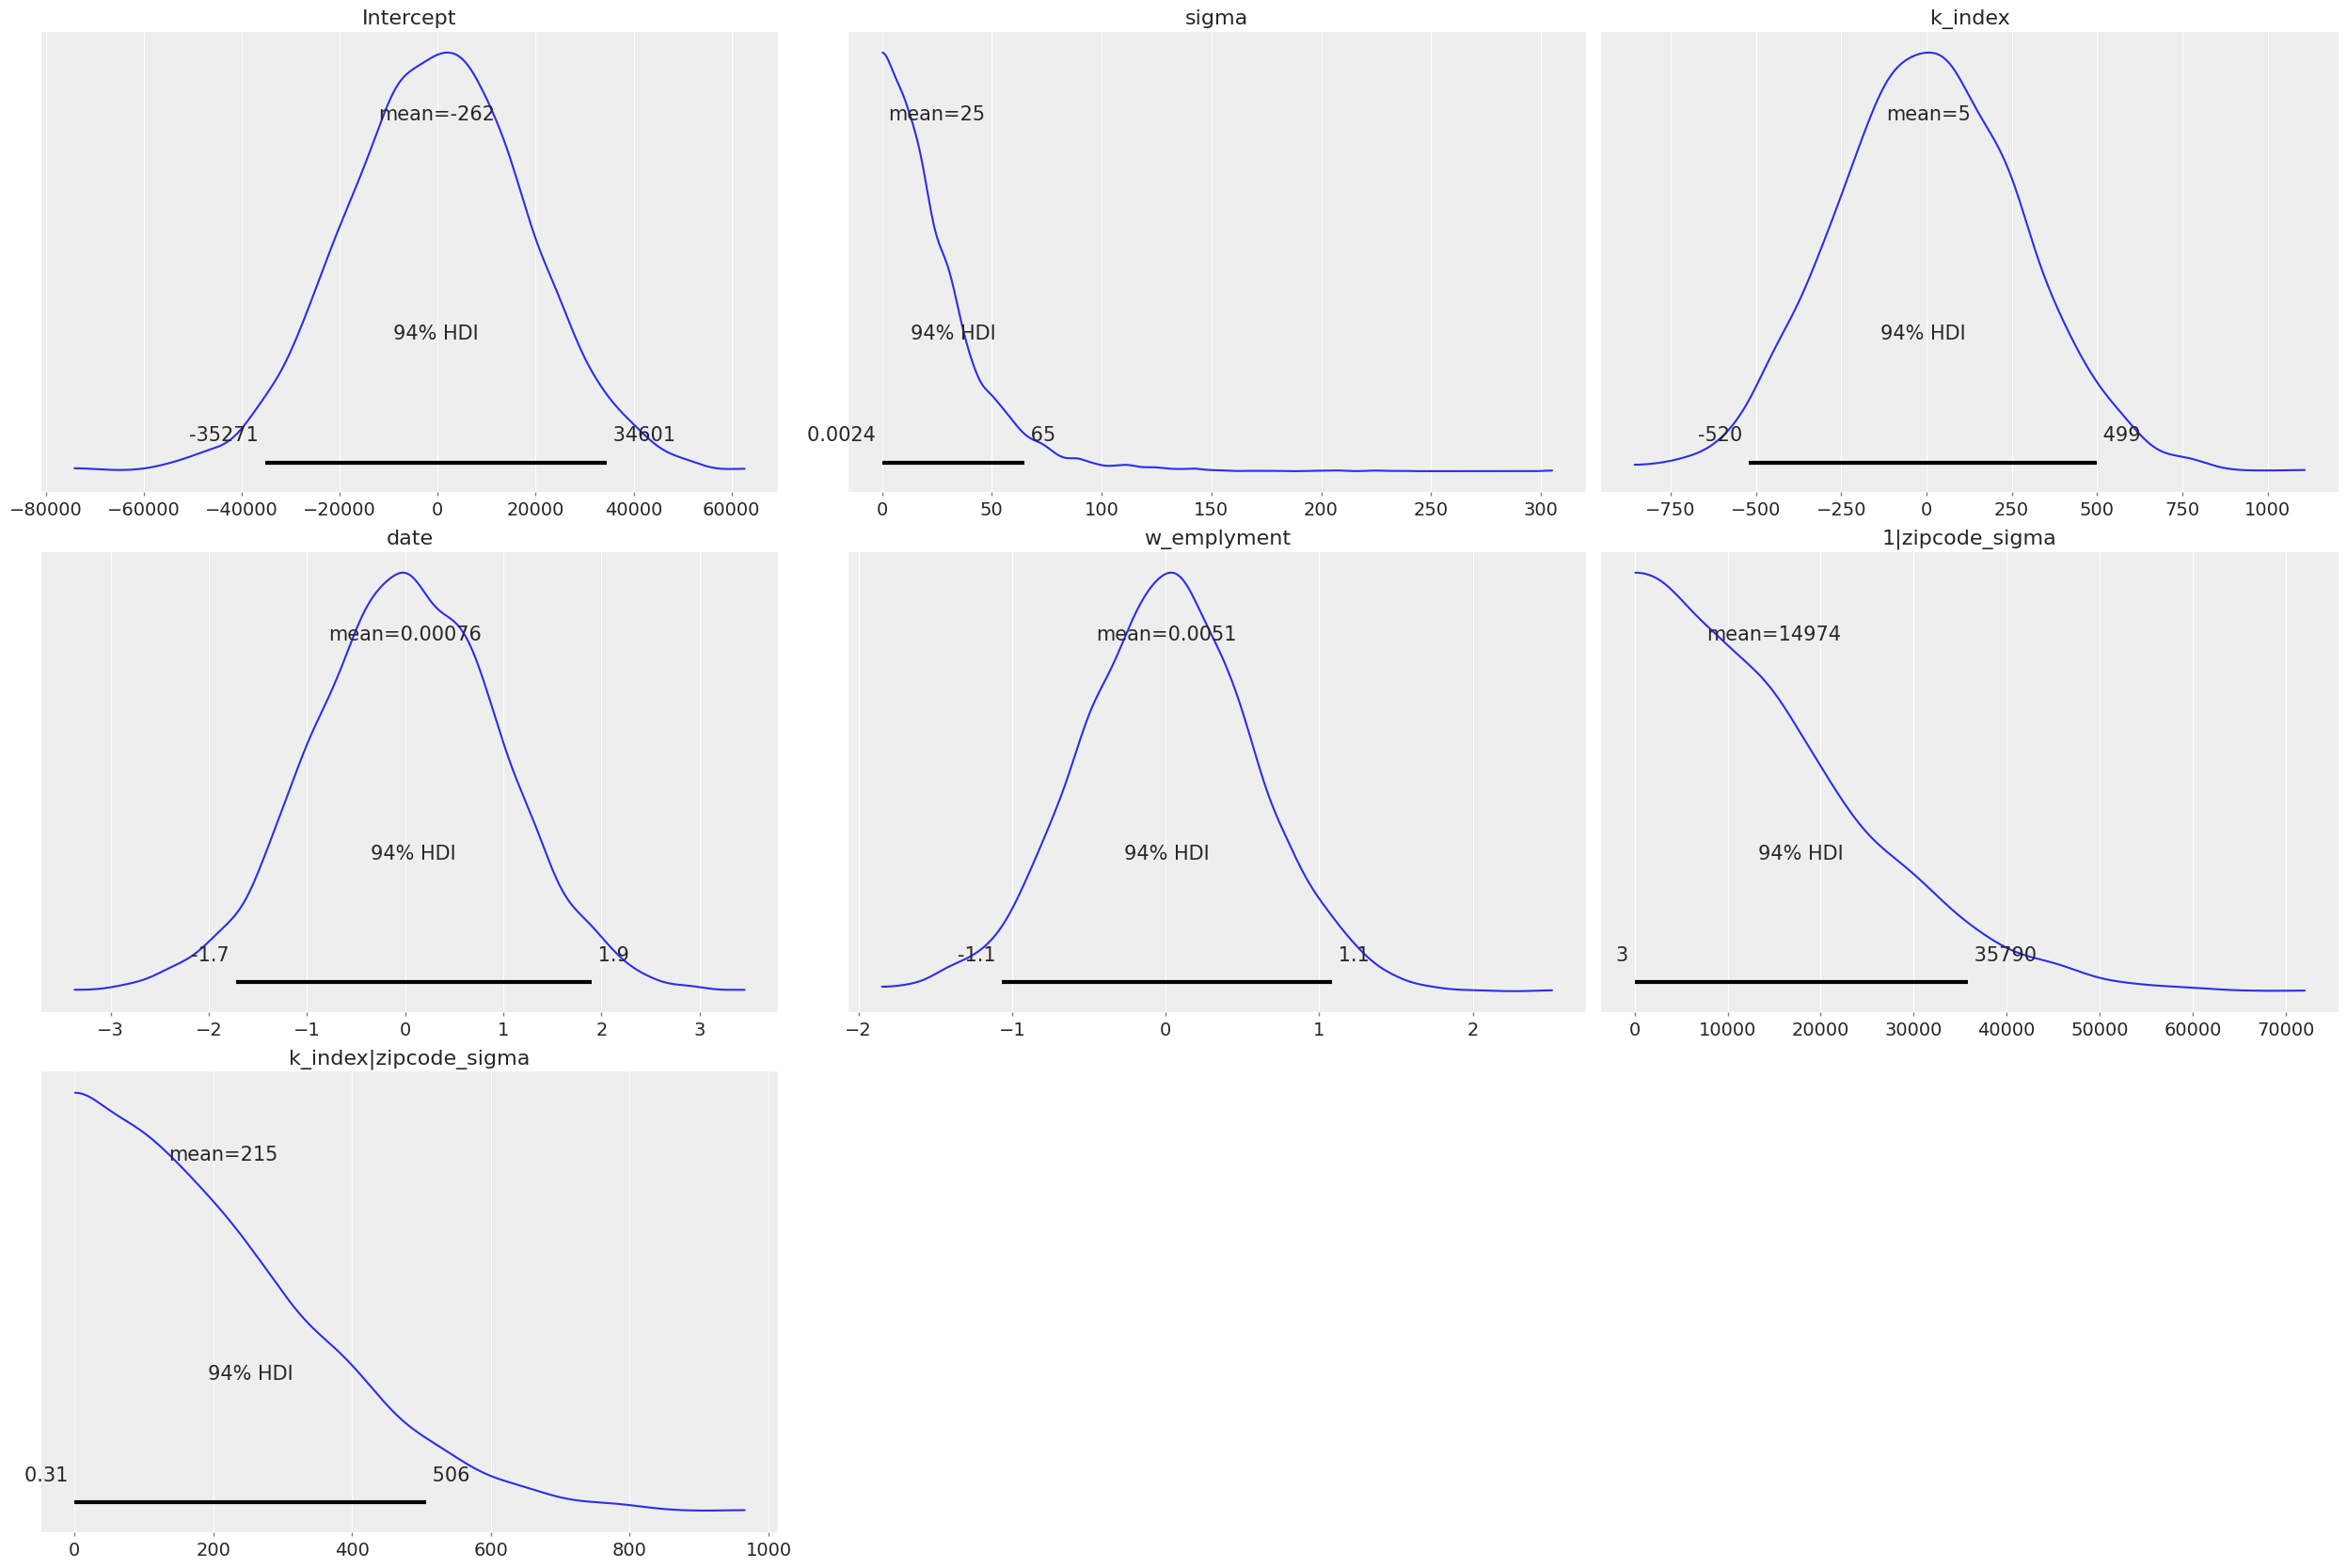
\includegraphics[width=\textwidth]{priori.png}
		\caption{Non-informative Priori used}
		\label{fig:priori}
	\end{minipage}
	\hfill
	\begin{minipage}[t]{0.48\textwidth}
		\centering
		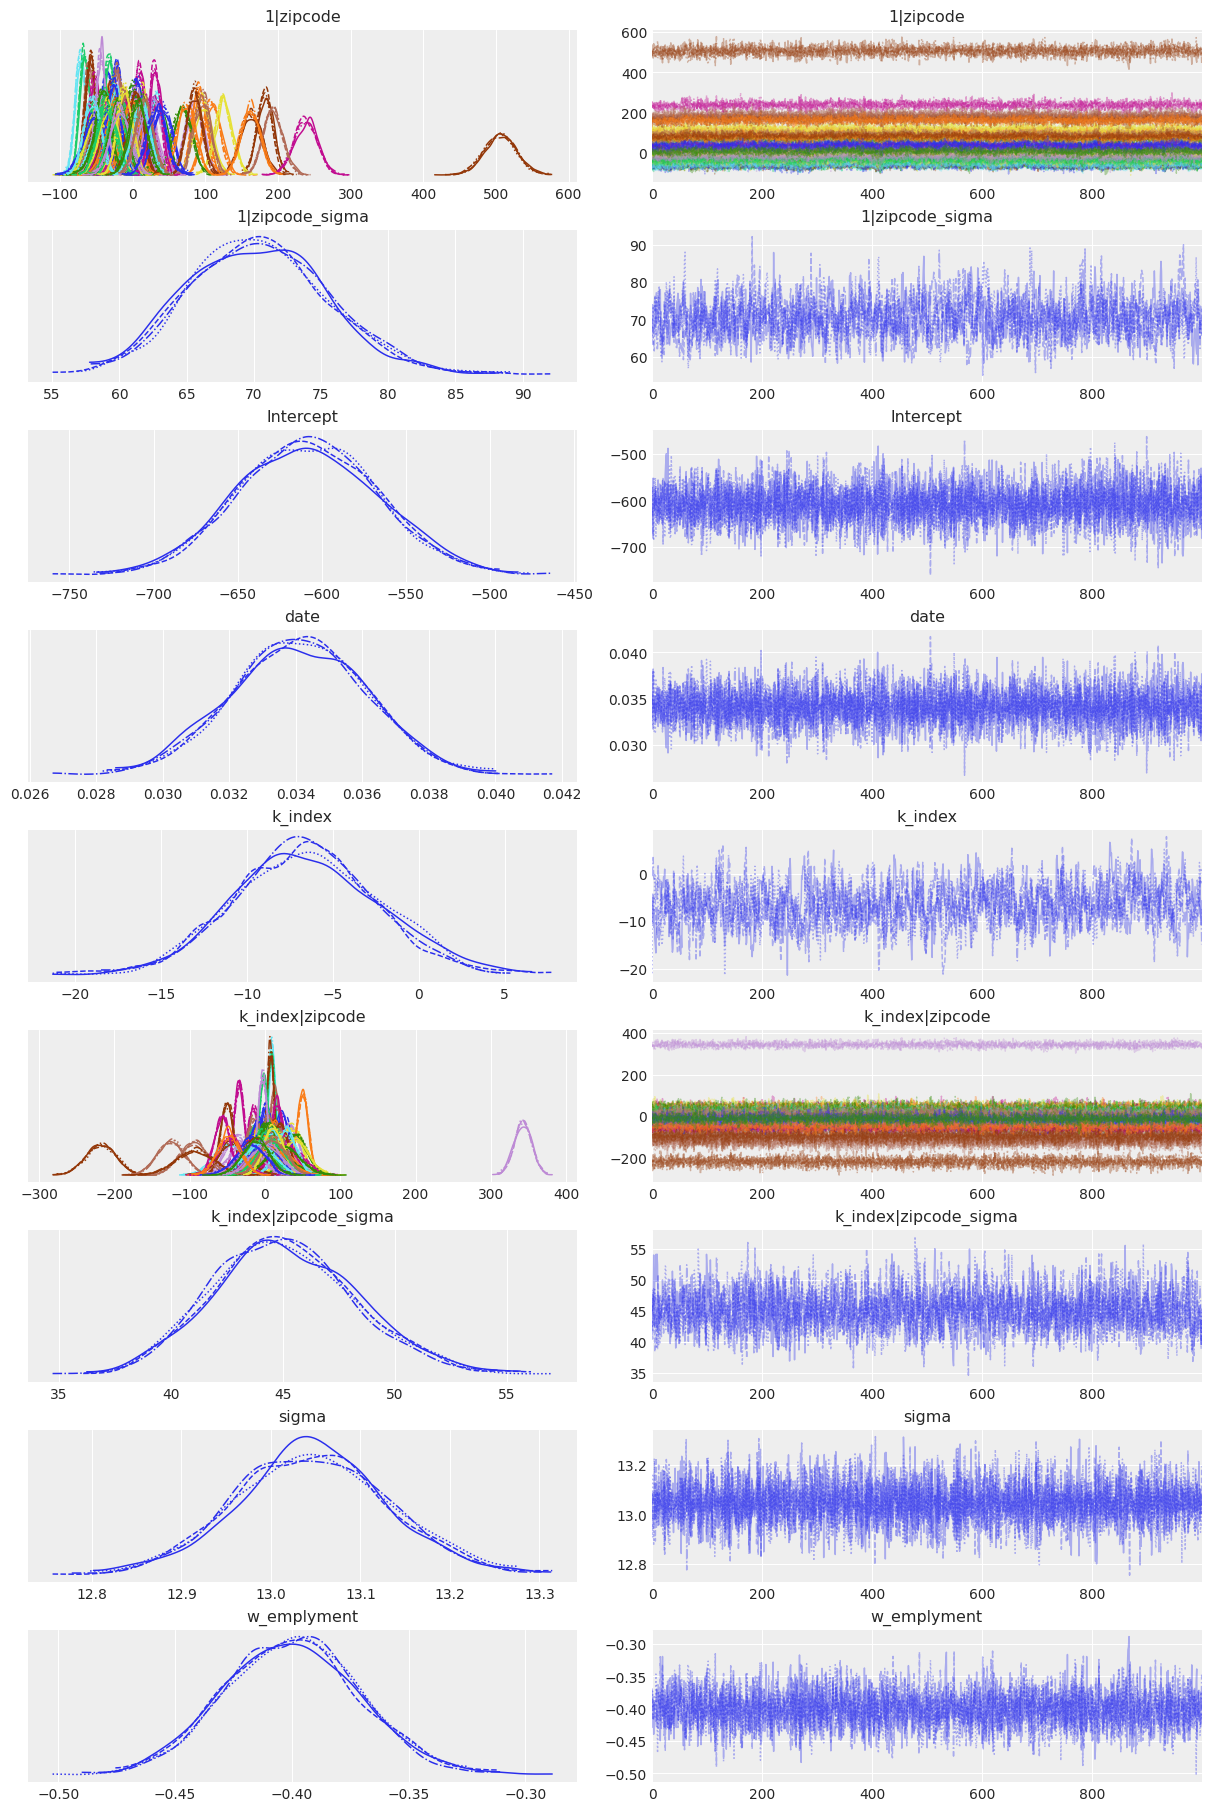
\includegraphics[width=\textwidth]{results.png}
		\caption{Summary of Regression Results}
		\label{fig:results}
	\end{minipage}
\end{figure}


\end{document}
